\documentclass[]{elsarticle} %review=doublespace preprint=single 5p=2 column
%%% Begin My package additions %%%%%%%%%%%%%%%%%%%
\usepackage[hyphens]{url}



\usepackage{lineno} % add
\providecommand{\tightlist}{%
  \setlength{\itemsep}{0pt}\setlength{\parskip}{0pt}}

\usepackage{graphicx}
\usepackage{booktabs} % book-quality tables
%%%%%%%%%%%%%%%% end my additions to header

\usepackage[T1]{fontenc}
\usepackage{lmodern}
\usepackage{amssymb,amsmath}
\usepackage{ifxetex,ifluatex}
\usepackage{fixltx2e} % provides \textsubscript
% use upquote if available, for straight quotes in verbatim environments
\IfFileExists{upquote.sty}{\usepackage{upquote}}{}
\ifnum 0\ifxetex 1\fi\ifluatex 1\fi=0 % if pdftex
  \usepackage[utf8]{inputenc}
\else % if luatex or xelatex
  \usepackage{fontspec}
  \ifxetex
    \usepackage{xltxtra,xunicode}
  \fi
  \defaultfontfeatures{Mapping=tex-text,Scale=MatchLowercase}
  \newcommand{\euro}{€}
\fi
% use microtype if available
\IfFileExists{microtype.sty}{\usepackage{microtype}}{}
\usepackage[margin=1in]{geometry}
\bibliographystyle{elsarticle-harv}
\usepackage{longtable}
\ifxetex
  \usepackage[setpagesize=false, % page size defined by xetex
              unicode=false, % unicode breaks when used with xetex
              xetex]{hyperref}
\else
  \usepackage[unicode=true]{hyperref}
\fi
\hypersetup{breaklinks=true,
            bookmarks=true,
            pdfauthor={},
            pdftitle={Modelling Risk and Uncertainty in Flood-based Farming Systems using a Knowledge-based Approach.},
            colorlinks=true,
            urlcolor=blue,
            linkcolor=blue,
            pdfborder={0 0 0}}
\urlstyle{same}  % don't use monospace font for urls

\setcounter{secnumdepth}{5}
% Pandoc toggle for numbering sections (defaults to be off)


% Pandoc header
\usepackage{setspace}\setstretch{1.5}
\usepackage{float} \floatplacement{figure}{H}
\newcommand{\beginsupplement}{\setcounter{table}{0}
\renewcommand{\thetable}{S\arabic{table}} \setcounter{figure}{0}
\renewcommand{\thefigure}{S\arabic{figure}}}



\begin{document}
\begin{frontmatter}

  \title{Modelling Risk and Uncertainty in Flood-based Farming Systems using a Knowledge-based Approach.}
    \author[KU,ICRAF]{Issoufou, Liman Harou\corref{Corresponding Author}}
   \ead{issoufoul@gmail.com; L.issoufou@cgiar.org} 
    \author[INRES]{Cory Whitney}
   \ead{cory.whitney@uni-bonn.de} 
    \author[KU]{James Kung'u}
   \ead{kungu.james@ku.ac.ke} 
    \author[INRES]{Eike Luedeling}
   \ead{luedeling@uni-bonn.de} 
      \address[KU]{Kenyatta University, Department of Environmental Sciences, P.O. Box 43844 00100 Nairobi, Kenya}
    \address[ICRAF]{World Agroforestry Centre (ICRAF), United Nations Avenue, Gigiri, P.O. Box 30677-00100, Nairobi, Kenya}
    \address[INRES]{University of Bonn, Department of Horticultural Sciences, Auf dem Hügel 6, D-53121, Bonn, Germany}
    \address[ZEF]{Center for Development research (ZEF), University of Bonn, Genscherallee 3, D-53113, Bonn, Germany}
    
  \begin{abstract}
  Modelling the performance of crops grown under specific conditions is an important strategy to support agricultural decisions. Towards this end, many crop models are being used to inform agricultural policies. However, many of these models are applied beyond a reasonable scope of application, mainly because they are either designed for other settings, they fail to capture system complexity, or because some of their data requirements are not within reach. This work attempts to address these challenges by deriving a crop model using a set of probabilistic methods rooted in Decision Theory. We transparently use all available sources of information and consider all relevant uncertainties using participatory analysis. The transdisciplinary process results in a model where all important variables and their interactions, as determined by calibrated experts and relevant literature, are used to simulate the plausible ranges of expected grain and biomass yield at various stages of crop development. System components are described using individual Bayesian networks, in which expert knowledge is used to specify causal relationships among important variables along with their probability distributions. These Bayesian networks, along with other quantitative variables, are used as inputs to Monte Carlo models that simulate the plausible performance of crops. Our objective is to develop a customizable solution-oriented approach to crop modelling in settings where data and resources are limited. We describe how such a model can be developed and provide some applications in three case studies focusing on flood-based farming systems. The case studies illustrate the scope of such a model by assessing the performance of a cropping system, individual crops, or other factors of high agricultural importance across the Tigray region of Ethiopia and Kisumu County of Kenya. The present supporting material provides further details on some of the aspects briefly described in the main paper. These aspects, mainly, are the different modules and sub-modules that make up the generic model. Still, this material will only give a general idea about the model. The full model is provided as reproducible code in two repositories available on GitHub. The \href{https://github.com/Issoufou-Liman/decisionSupportExtra}{first one} is a package describing all functions used for various purposes such as translating the expert-elicited data into graphical computer models, extracting local Bayesian networks, sampling from the joint distribution of these Bayesian networks based on a specific query, constructing estimates (as defined in the \emph{decisionSupport} package) from Bayesian networks for Monte Carlo simulations, or plotting the results. \href{https://github.com/Issoufou-Liman/Modelling_FBFS}{The second} is an Rmarkdown folder containing the necessary ingredients to reproduce the main paper and these supplementary materials.
  \end{abstract}
  
 \end{frontmatter}

\beginsupplement

\hypertarget{introduction}{%
\section*{Introduction}\label{introduction}}
\addcontentsline{toc}{section}{Introduction}

Crop modelling has been used to provide guidance to scientists and decision makers on various aspects of agriculture. Several of these crop models were developed to assess aspects of high agricultural importance (e.g.~soil water, soil carbon, crop growth, crop yield under constraints). Despite their usefulness and widespread use across the globe, there are often concerns about several aspects, such as the requirement for precise data, which are largely unavailable, or the complexity of the system being modelled.
This work attempts to address these concerns by using a set of Decision Theory methods to propose a new approach to crop modelling. We use all available sources of information to develop a generic crop model for flood-based farming systems (FBFS) by fusing Bayesian networks (BNs) and Monte Carlo models. BNs are used to include qualitative variables, whereas MC models were used for quantitative ones. We describe how such a model can be developed and provide ways for deriving customized models for specific situations using three case studies. Each case study presents a customized instance of the generic model to demonstrate the usefulness and usability of the model from different perspectives. The modelling exercise took place in Kisumu County in Kenya and the Tigray region in Ethiopia. This document provides supplementary materials supporting the main paper. The details provided here concern, mainly, the different modules and sub-module that make up the generic model. Still, this material will only give a general idea about the model. The full model is provided as reproducible code in two repositories available on GitHub. \href{https://github.com/Issoufou-Liman/decisionSupportExtra}{The first one} is a package describing the different functions. \href{https://github.com/Issoufou-Liman/Modelling_FBFS}{The second} is an Rmarkdown folder containing the necessary ingredients to reproduce the main paper and this supplementary material.

\hypertarget{data-collection-process-and-information-extraction}{%
\section{Data collection process and information extraction}\label{data-collection-process-and-information-extraction}}

The data collection was conducted in five sequential steps used to maximize information gain along the process. We started with an extensive literature review which covered most of the database of the flood-based livelihood network foundation and extended to other sources. From this review, we designed broad leading questions and conducted expert interviews aiming at general discussions on the topic of FBFS. The outcomes of these interviews were generated as text files documenting the expert reasoning. Note that these interviews were conducted with individual experts either via skype or as physical meeting and no structure was imposed. The expert was first brief on the objective of the study and asked one simple question: How do you define FBFS? The remaining discussions were mainly dictated by the aspects considered in the definition given by the expert. In many cases, the experts expanded on the importance of flooding systems (set of infrastructures farmers used to facilitate flooding of their fields such as the canals) and the water source. Some of the recurrent follow-up questions concerned the importance of the flooding systems in FBFS, or which type of water source makes FBFS sustainable. These high-level discussions were followed by a set of focus group discussions.
The focus group discussions were conducted on the considered FBFS schemes with small groups (3 -- 5 people per group) of knowledgeable people and a well-trained enumerator whose tasks were to moderate the discussions and take notes of farmers' narratives. These knowledgeable people were represented by key farmers, farmers' representatives, and technicians working with them. The discussions started with an overview of agriculture to mainly focus on the importance of FBFS in the area. The local practices of FBFS were described in terms of flooding systems, crop types, cropping systems, and socio-institutional arrangements in place. Where we had several groups, the discussions were first conducted in subgroups, then in a group with all farmers. These group discussions also resulted in text files documenting the most important points of each discussion.
The focus group discussions were followed by local expert consultations, whose goal was to examine the information from the focus group and high-level discussions, enrich the concepts that arose, and ultimately draft a model. The consultation process started with an overview of decision analysis followed by a calibration training. The experts were then briefed on the information acquired in the previous steps and provided with further sources of information (e.g.~global yield gap database, FBLN database). After defining the main modules of the model, the experts were engaged in participatory model development in working groups. The experts first drafted the graphical model, then estimated the variable values. At this stage, separate models were drafted for both Kisumu County and Tigray.
The next step consisted of farmer interviews, which focused on the estimation of yield values and the enumeration of farming constraints. The farmers were informed about the meaning of the 90\% confidence interval, the uniform distribution, and asked to estimate the ranges (5\% and 95\% quantiles) of yield values they had achieved on their farm over the last ten years. They were then asked to list the most important constraints that affect crop yield on their farms. Based on recommendations from key informants, the farmers were selected based on their wealth status (i.e.~poor farmers, average farmers, and rich farmers) considering a stratified sampling. We considered three groups of farmers in a stratified sampling. Based on these constraints and the other information summarized in the two models, these models were further merged into a single model that captured the realities of both study regions at the Center for Development Research (ZEF), University of Bonn, Germany.

\hypertarget{refs1}{%
\section{Description of the modules in the BN model}\label{refs1}}

\hypertarget{refs11}{%
\subsection{Farming constraints at farming plot level}\label{refs11}}

The purpose of the BNs is to describe the node `farming constraints' (FarmConstraints), which accounts for all limiting factors deemed important to FBFS in the study areas. The most important limiting factors describing the farming constraints in the study areas (Figure \ref{fig:fig1}) are the adequacy of water supply to crops (AdeqWatSupl), the effectiveness of cropping systems (EffCropSystems), and the quality of farming practices (AgricManagEff) resulting from farmers' managements options (Figure \ref{fig:fig2} to Figure \ref{fig:fig6}). These were described in three modules: the soil water, the cropping system and the management modules. They are described in more detail in sections \ref{refs12} to \ref{refs14}.

\begin{figure}[!h]

{\centering 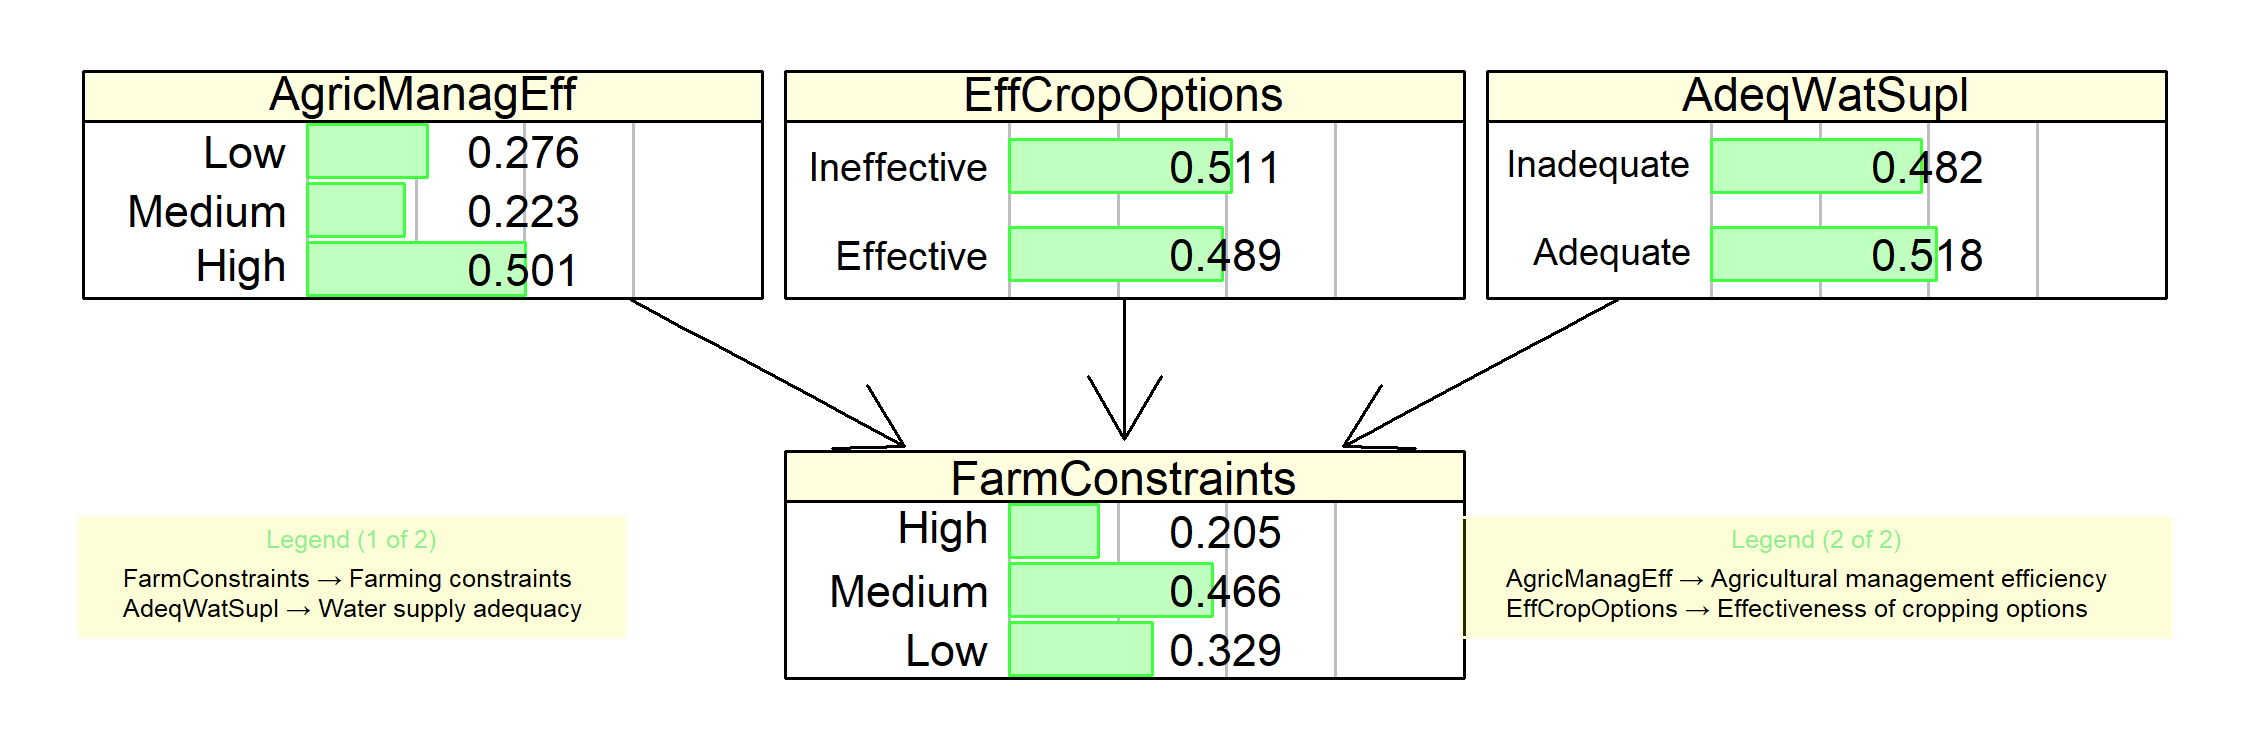
\includegraphics[width=1\linewidth,]{figures/figure_s1} 

}

\caption{Bayesian Network describing important variables as part of a mixed model describing the farming constraints in flood-based farming systems in Kenya and Ethiopia.}\label{fig:fig1}
\end{figure}

\hypertarget{refs12}{%
\subsection{Water supply adequacy}\label{refs12}}

Because of the complexity of water supply in FBFS, water supply adequacy was described via 2 sub-modules (Figure \ref{fig:fig2}; Figure \ref{fig:fig3}). The amount of floodwater reaching the farming plot (FloodReachsPlot) was assessed separately, since it is an important variable with regard to the overall available water for crop development in FBFS settings.

\begin{figure}[!h]

{\centering 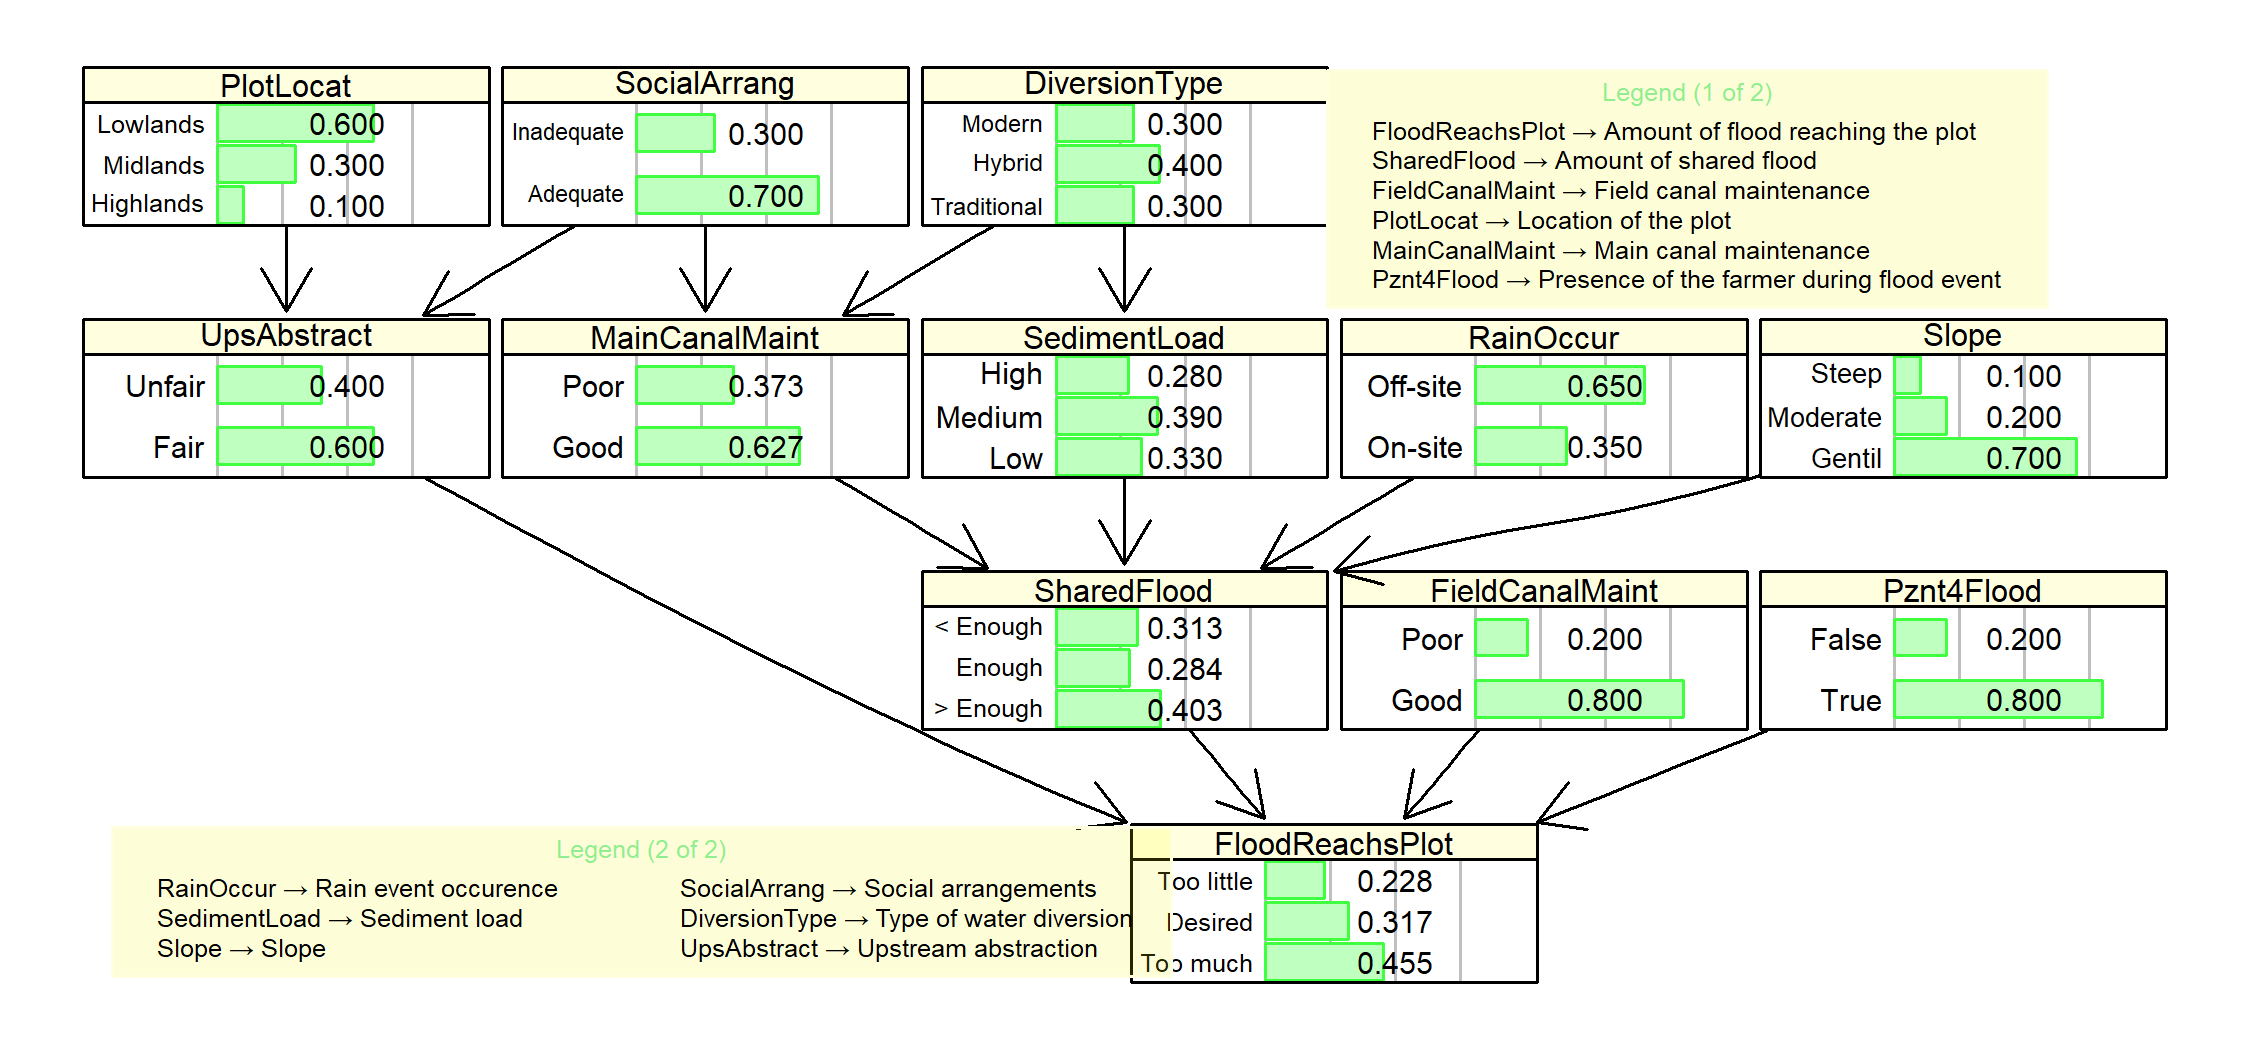
\includegraphics[width=1\linewidth,]{figures/figure_s2} 

}

\caption{Bayesian Network describing important variables as part of a mixed model describing the amount of floodwater at the farming plot level in FBFS in Kenya and Ethiopia.}\label{fig:fig2}
\end{figure}

At the root of the BN that describes the amount of floodwater reaching the plot are the nodes describing water diversion type (DiversionType), the social arrangement for water acquisition and sharing (SocialArrang), and the location of the farming plot (PlotLocat). The water diversion type is important, since it determines the overall water delivery (SharedFlood) and ultimately the overall expected flood amount at the plot level (FloodReachsPlot). It acts via the way in which farmers are committed as a group (SocialArrang) to maintain their main water distribution networks (MainCanalMaint) and its efficiency with regard to sediment load (SedimentLoad). If the social organisation (SocialArrang) is not adequate along a topographic gradient (Slope), this may lead to unfair upstream abstraction (UpsAbstract), hence penalising water users downstream (FloodReachsPlot). Flood water is trapped in FBFS fields using earthen bunds, which need to be opened at the right time either for irrigation, or for water release, if there is too much water. Individual farmers, therefore, need to make sure this happens by being present at the right time and making sure the water is diverted from the main canal to the respective secondary and tertiary sub-divisions of their water distribution system. Given the adequacy of the above-mentioned aspects, the presence of the farmers in the field during floods (Pznt4Flood) and the quality of canal maintenance (FieldCanalMaint) can still strongly affect the amount of floodwater reaching the plot (FloodReachsPlot), and ultimately the overall soil water budget. The presence of the farmer and the quality of canal maintenance can either have minor importance when it rains on the field (RainOccur = On-site) or major importance in the case of spontaneous flood events from upstream (RainOccur = Off-site).

\begin{figure}[!h]

{\centering 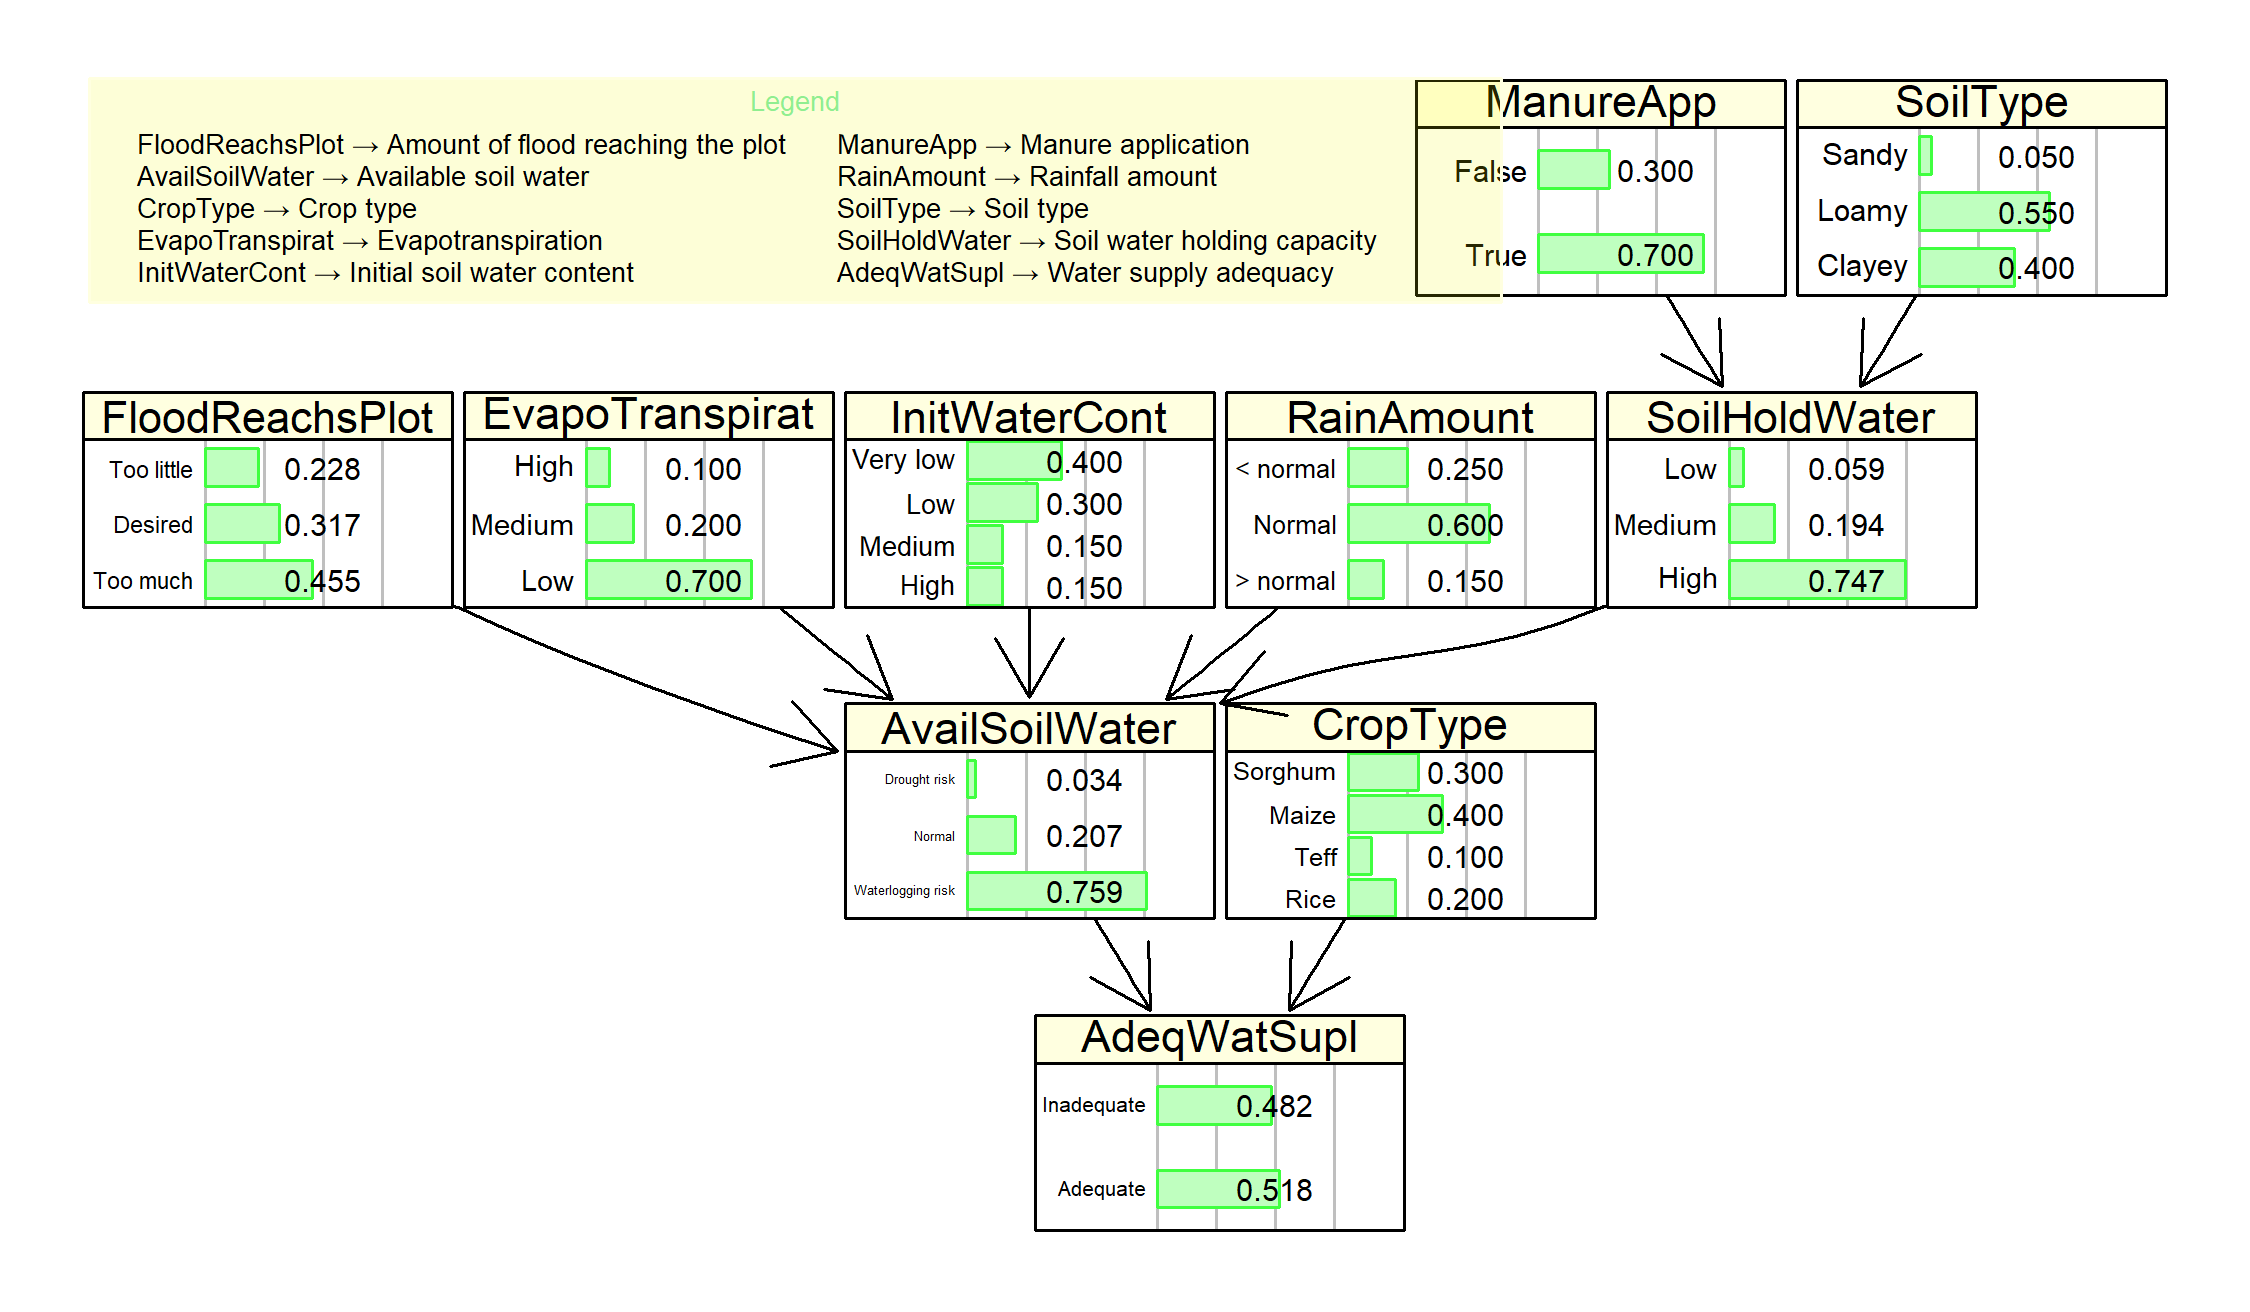
\includegraphics[width=1\linewidth,]{figures/figure_s3} 

}

\caption{Bayesian Network describing important variables as part of a mixed model describing the available soil water content in flood-based farming systems in Kenya and Ethiopia.}\label{fig:fig3}
\end{figure}

The soil water profile of a given farming plot includes important biophysical aspects related to soils and climate. The available water for crops is determined by the soil water holding capacity (SoilHoldWater), the total amount and temporal distribution of rainfall (RainAmount) and residual soil moisture (InitWaterCont), which can be significant under certain FBFS, such as flood recession agriculture. Soil water holding capacity (SoilHoldWater) can vary greatly depending on the soil type (SoilType) and the soil management strategies employed by the farmer (e.g.~manure application; ManureApp).

\hypertarget{refs13}{%
\subsection{Agricultural management efficiency}\label{refs13}}

Agricultural management efficiency (AgricManagEff) is described using two submodules (Figure \ref{fig:fig4}; Figure \ref{fig:fig5}): one describing the availability of soil nutrients (AvailSoilNut), and another describing the overall agricultural management efficiency. The availability of soil nutrients is defined by fertilizer applications either in the form of organic (ManureApp) or mineral additions (FertiApp) by the farmer, and on the other hand by the sediment naturally brought by the flood water. Here, it is important to distinguish between coarse sediments (SedimentLoad) described under the rubric Available soil water, which are likely to have negative impacts, and the fine rich sediments (AddSediments), which have positive impacts on crops. Fertilizer application can only be expected when the fertilizer desired by the farmer is available on the market at the time when the farmers can afford it (Access2Inputs). This depends on the purchasing power of farmers and their willingness to acquire the fertilizers (RelativeWealth), as well as on mutual assistance (MutualAids) among farmers.

\begin{figure}[!h]

{\centering 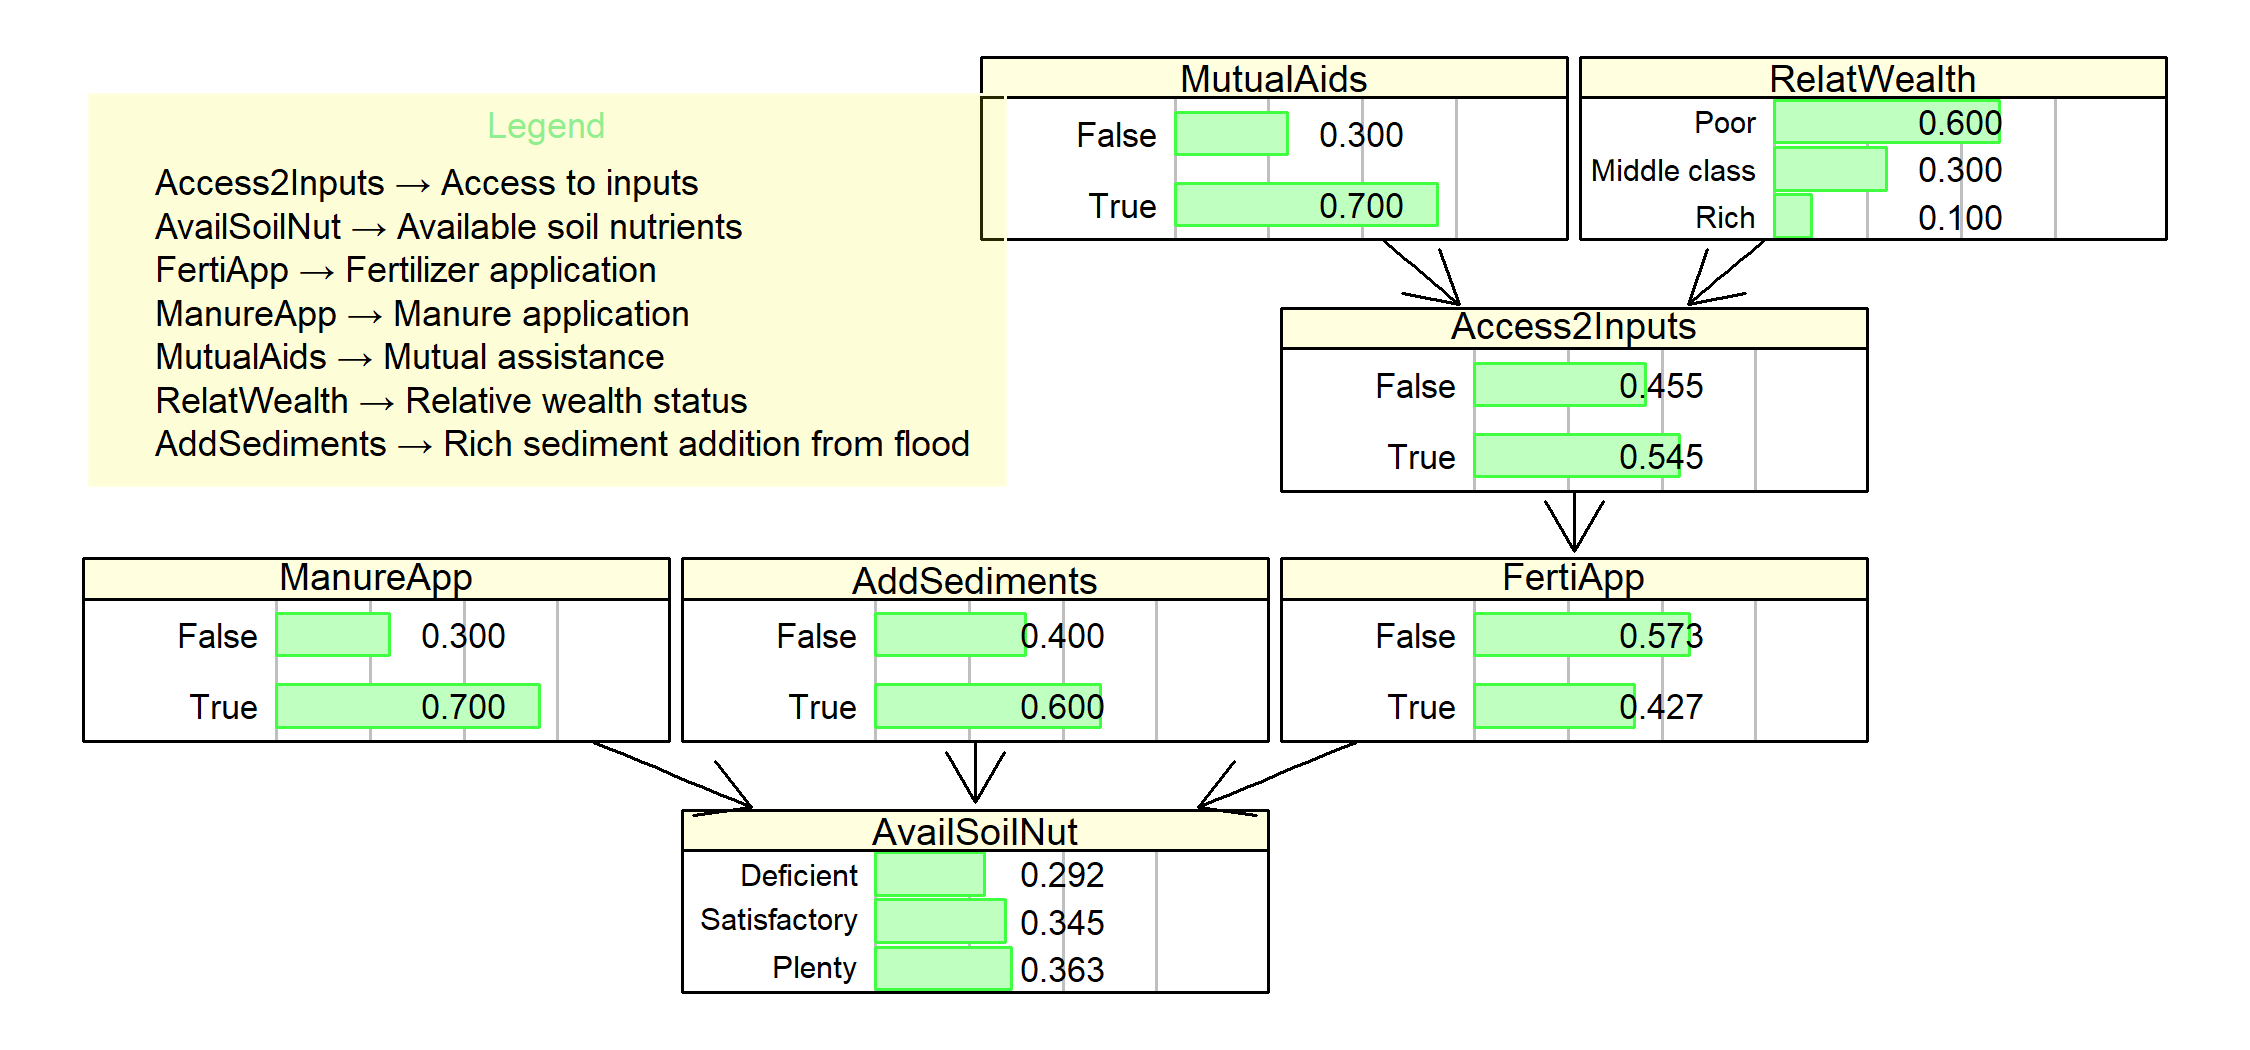
\includegraphics[width=1\linewidth,]{figures/figure_s4} 

}

\caption{Bayesian Network describing important variables as part of a mixed model describing the available nutrients in flood-based farming systems in Kenya and Ethiopia.}\label{fig:fig4}
\end{figure}

\begin{figure}[!h]

{\centering 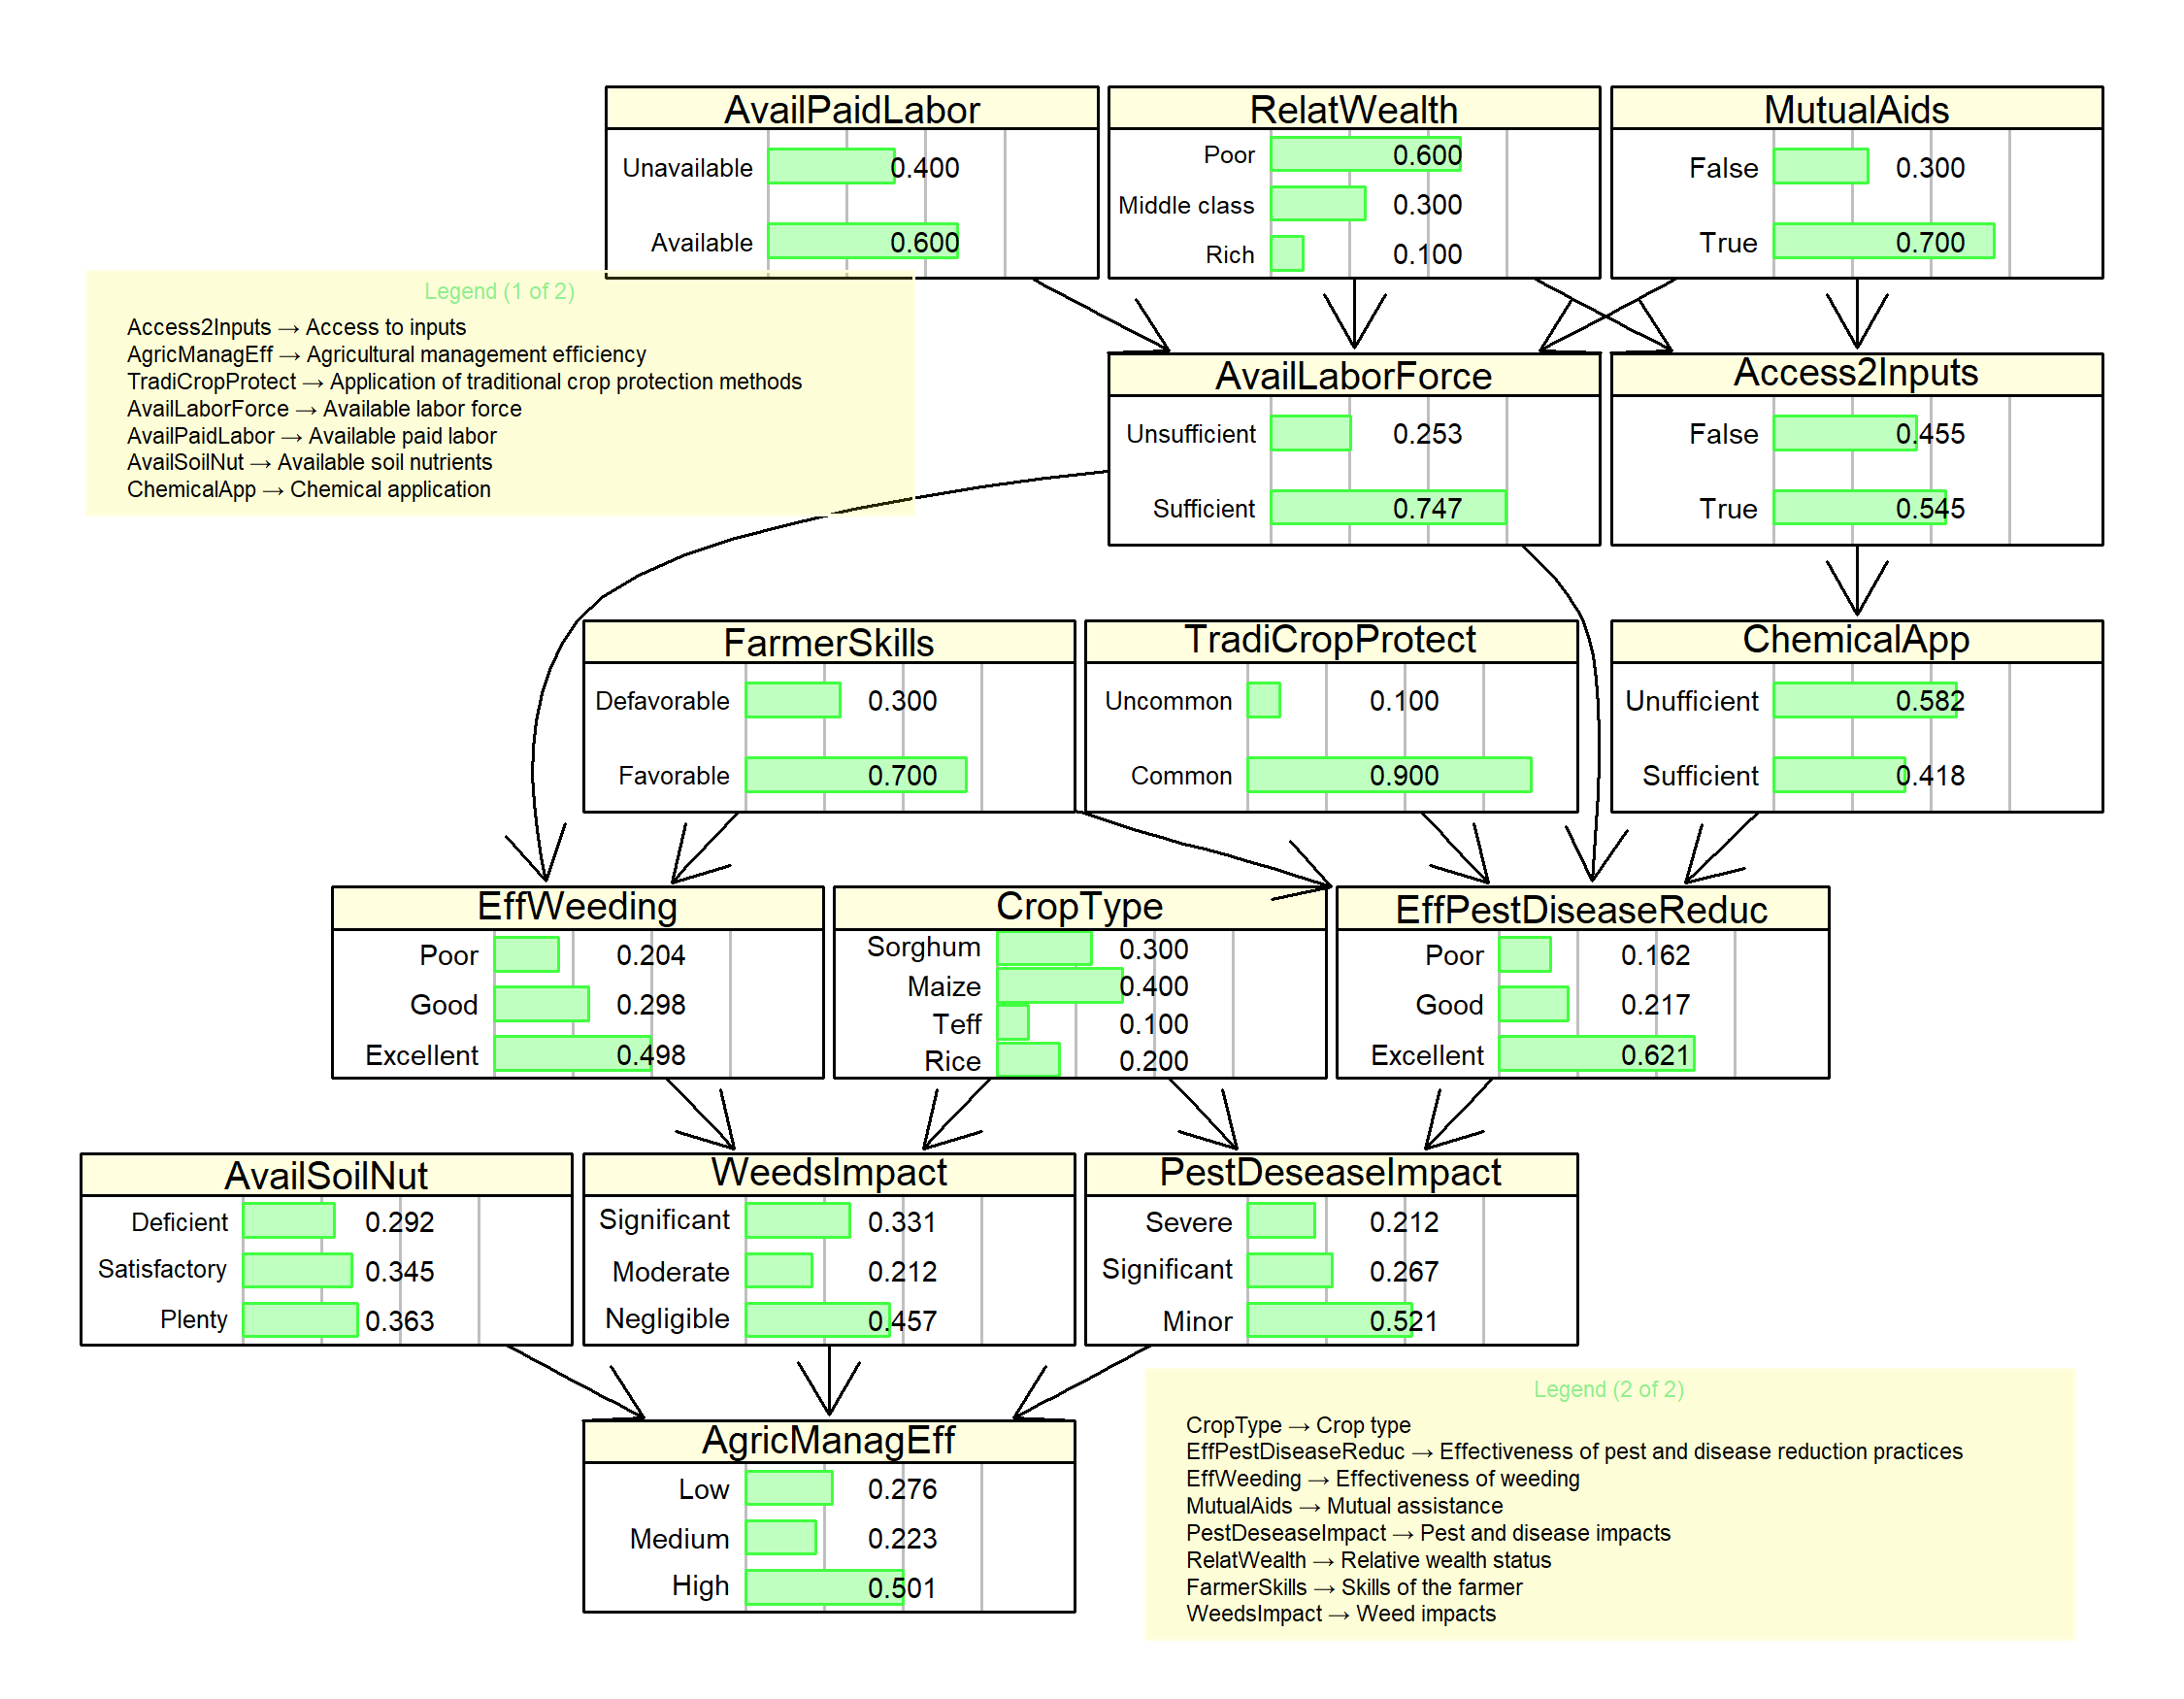
\includegraphics[width=1\linewidth,]{figures/figure_s5} 

}

\caption{Bayesian Network describing important variables as part of a mixed model describing the effectiveness of agricultural management in flood-based farming systems in Kenya and Ethiopia.}\label{fig:fig5}
\end{figure}

The factors of agricultural management efficiency include the available soil nutrients (AvailSoilNut), crop exposure/sensitivity to pests and diseases (PestDiseaseImpact) and the severity of weeds (WeedsImpact). The magnitude and recurrence of damage to crops due to pests \& diseases and yield losses due to weeds can be related to the skills of the farmers (FarmerSkills) in crop protection, the farmers' ability to acquire chemicals, and other aspects such as the available labour force, which may influence the effectiveness of crop protection.

\hypertarget{refs14}{%
\subsection{Effectiveness of cropping options}\label{refs14}}

The `effectiveness of cropping options' (EffCropsOptions) BN describes the various factors shaping the cropping system at the very early stages of crop growth. Crops are defined by their type (CropType: rice (\emph{Oryza sativa}), maize (\emph{Zea mays}), sorghum (\emph{Sorghum bicolor}), tef (\emph{Eragrostis tef})), their variety (CropVariety) and the farmers' decision regarding which crops to grow and how to grow them (Intercropping). The decision of the farmer to grow a given type of crop and variety have strong yield implications.

\begin{figure}[!h]

{\centering 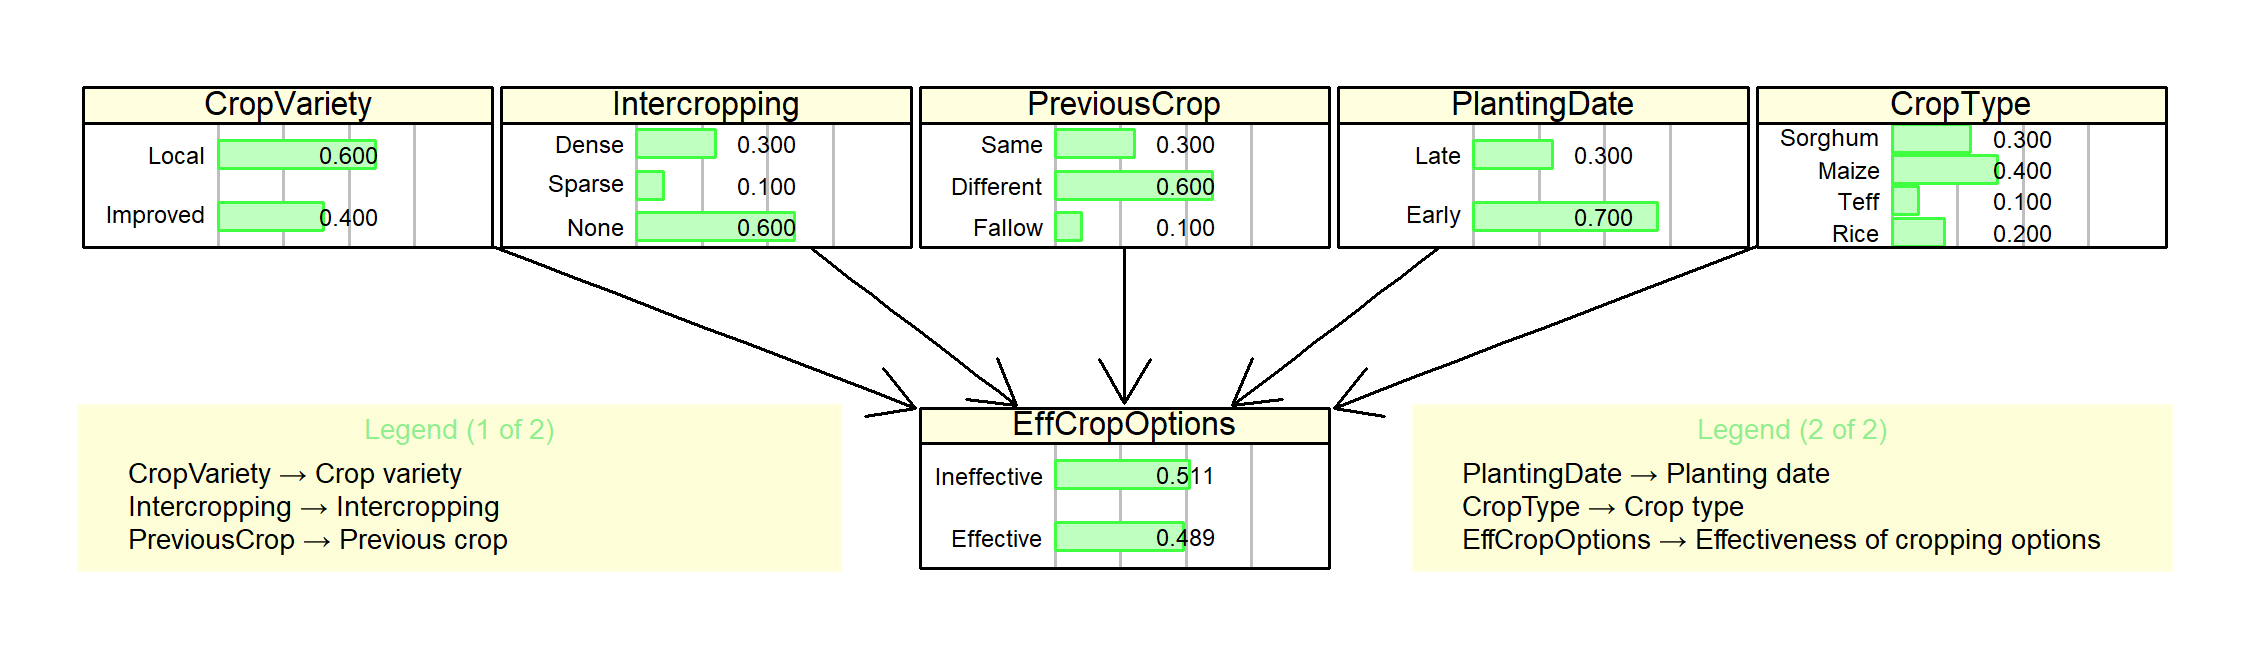
\includegraphics[width=1\linewidth,]{figures/figure_s6} 

}

\caption{Bayesian Network describing important variables as part of a mixed model of the effectiveness of cropping options in flood-based farming systems in Kenya and Ethiopia.}\label{fig:fig6}
\end{figure}

\hypertarget{refs2}{%
\section{BN structures and node sensitivity in relation to crop development}\label{refs2}}

The local BNs described above were connected to form a single BN accounting for the complexity of the farming system. This BN aims to integrate the joint effect of all farming constraints in one single variable (see section \ref{refs11}) to be used along with other variables described in the MC model. In the MC model, the entire BN was replicated with some changes in the CPTs and the causal relations when necessary. For example, the impact of weeds may depend on the crop development stage. The model assumes that crop sensitivity to biotic and abiotic factors depends on the period when these factors are considered. Therefore, these stage-specific BNs or rather the concepts embedded in their nodes, their causal relationships, and their CPTs were developed according to available information. BNs were developed to estimate the farming constraints at plot level and at each phenological stage of crop development. The BN nodes (Figure \ref{fig:fig1} to Figure \ref{fig:fig6}) are represented in the model in four crop development stages (e.g.~amount of shared flood at initial stage, development stage, mid stage, and late stage). A few BN nodes that are expected to remain constant (e.g.~the type of water diversion (DiversionType), the slope etc.), however, were represented only once in the model and transported through the various crop development stages. For example, the BN nodes `soil type' and `location of the farming plot' are considered static variables over time. They are unlikely to change, at least not within a few years, in contrast to other nodes such as the impact of weeds and diseases, which differs between consecutive phenological stages. We focus on processes at the initial stage in the description, but the target variable is assessed quantitatively at each of the four stages to feed the MC model.

\hypertarget{refs3}{%
\section{Quantitative assessment of Farming Constraints}\label{refs3}}

The inclusion of the farming constraints variable in the MC models requires its quantitative description capturing all possible scenarios for the variable. For each scenario, these estimates include the range of variable values spanning the 90\% confidence interval and its probability distribution as required by the \emph{mcSimulation} function (Luedeling et al., \protect\hyperlink{ref-Luedeling_Goehring_et_al_2019}{2019}). We generated the probabilities of the variable from the BN based on the query of interest. The resulting data were used to compute the lower bound, the median and the upper bound of the 90\% confidence interval, and to estimate the shape of the best-fitting probability distribution given several candidate distributions and the ranges of skewness and kurtosis (Cullen and Frey graph, also skewness-kurtosis plot) of the generated data (Cullen and Frey, \protect\hyperlink{ref-Cullen_and_Frey_1999}{1999}; Delignette-Muller and Dutang, \protect\hyperlink{ref-Delignette-Muller_and_Dutang_2015}{2015}). The probability distribution of the variable at the four crop development stages was assessed via visual observation of the Cullen and Frey graph (see example for the initial stage of crop development in Figure \ref{fig:fig7}).

\begin{figure}[!h]

{\centering 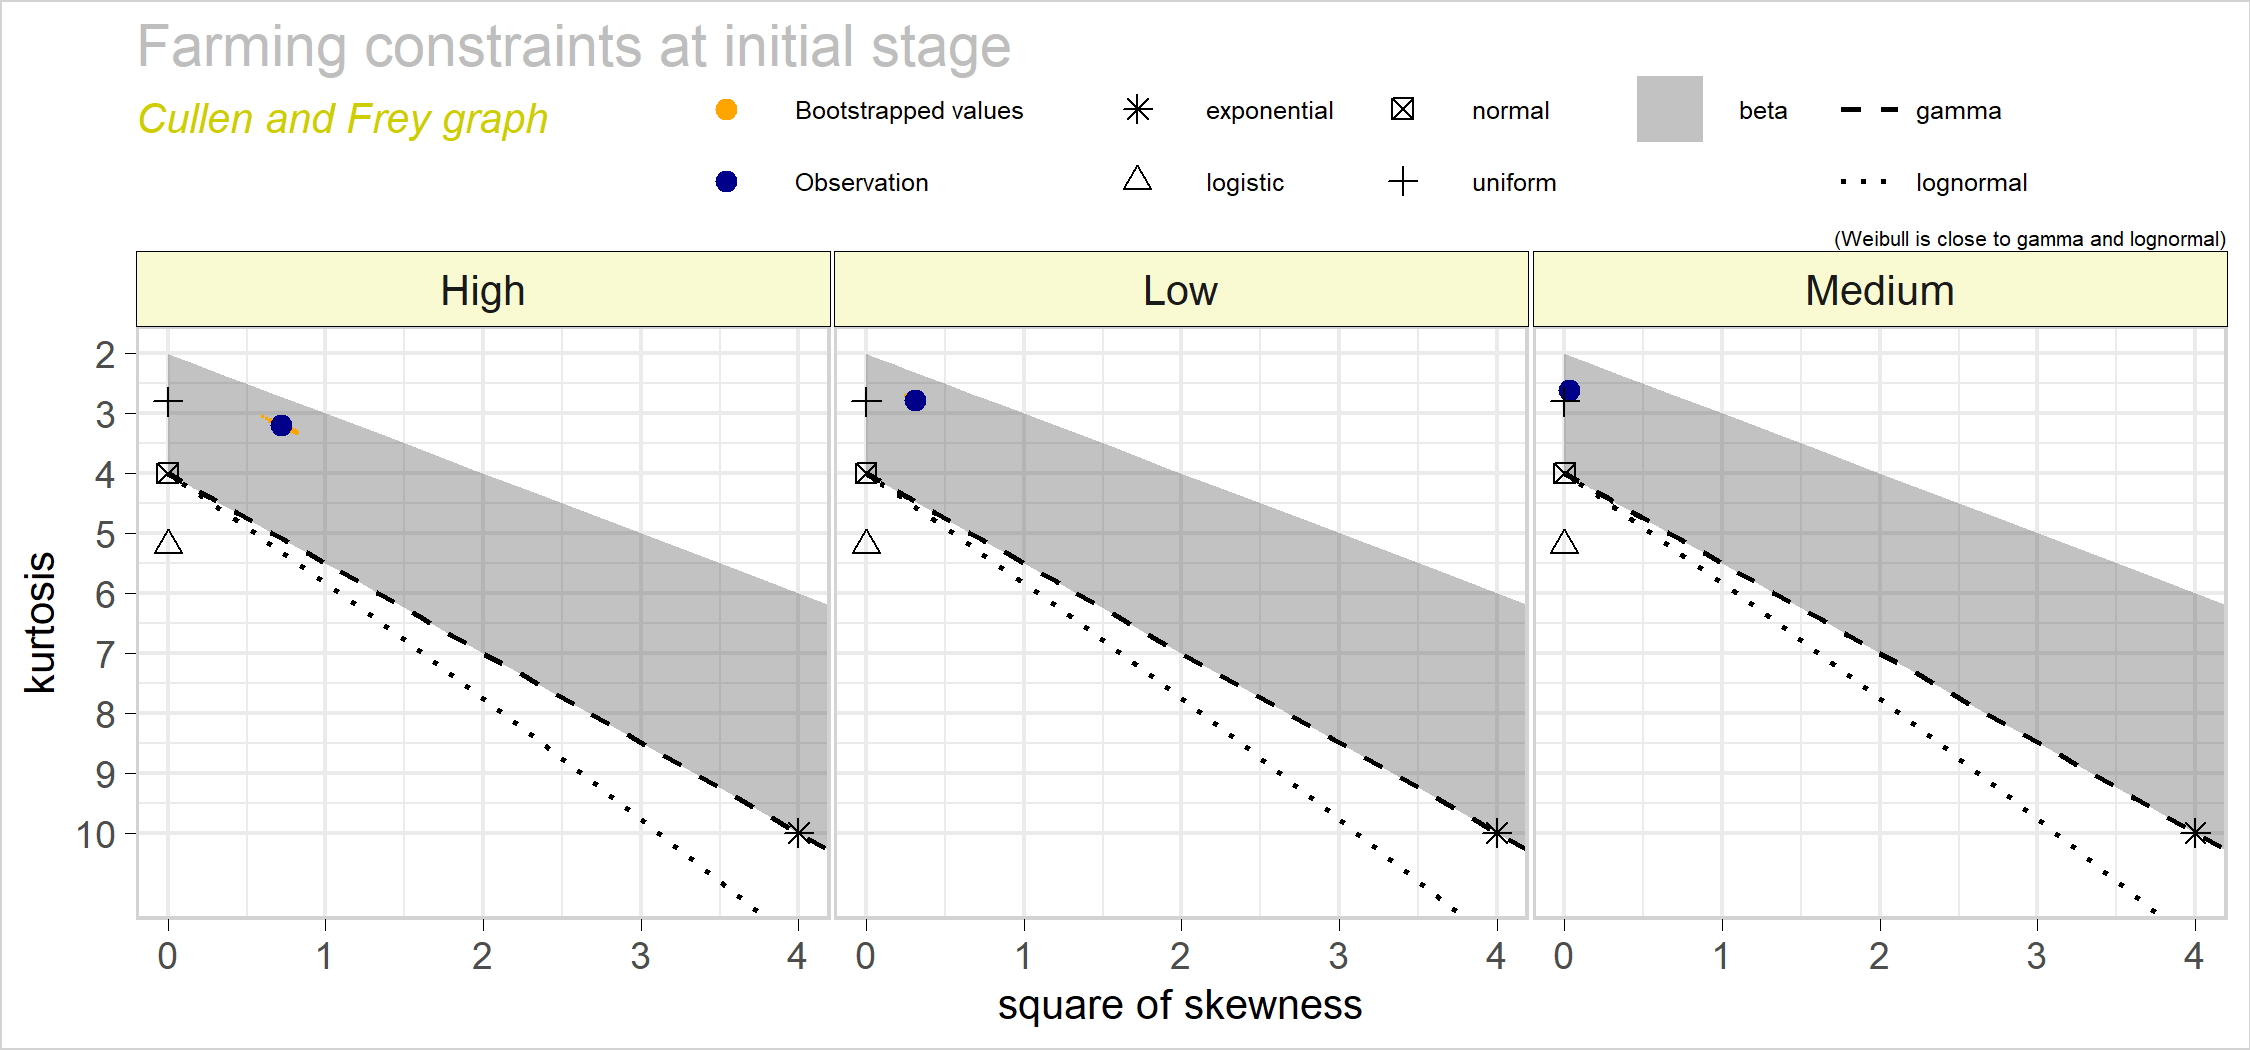
\includegraphics[width=1\linewidth,]{figures/figure_s7} 

}

\caption{Cullen and Frey graph showing the bounds for skewness and kurtosis and the best fitting distribution of three states of the variable ‘farming constraints’ derived from the joint distribution of a Bayesian network used to feed a Monte Carlo model as part of a mixed crop model for flood-based farming systems in Kisumu County (Kenya) and Tigray (Ethiopia). The Bayesian network describes the variable farming constraints at 4 crop development stages (i.e. initial, development, mid-season, and late stages). This figure provides an example for the initial stage.}\label{fig:fig7}
\end{figure}

\begin{figure}[!h]

{\centering 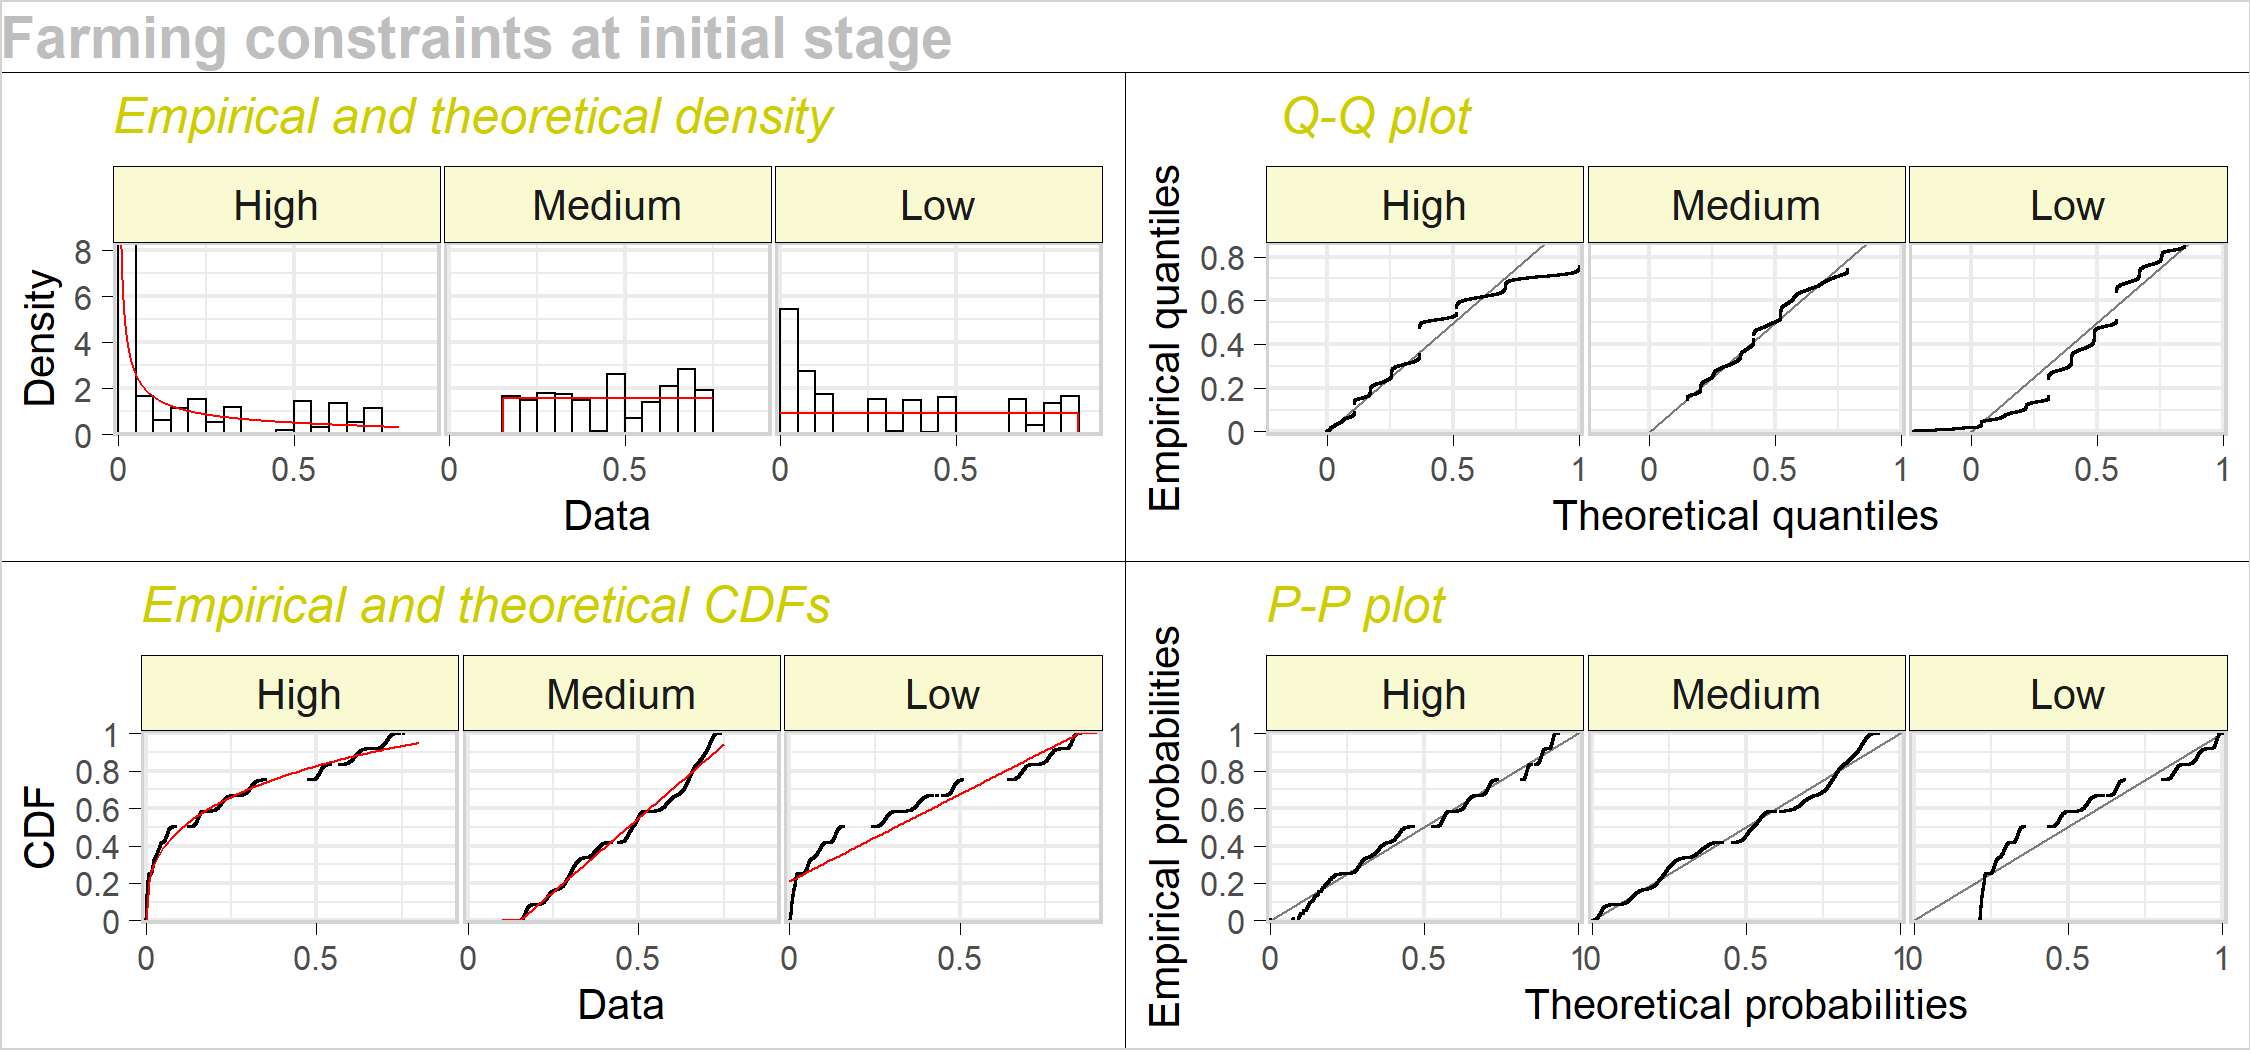
\includegraphics[width=1\linewidth,]{figures/figure_s8} 

}

\caption{Graphical assessment of probability distribution fits, including the quantile and probability plots along with the theoretical and empirical density and cumulative distribution functions, for the variable farming constraints derived from the joint distribution of a Bayesian network used to feed a Monte Carlo model as part of a mixed crop model for flood-based farming systems in Kisumu County (Kenya) and Tigray (Ethiopia). The Bayesian network describes the variable farming constraints at 4 crop development stages (i.e. initial, development, mid-season, and late stages). This figure provides example for the initial stage.}\label{fig:fig8}
\end{figure}

The best fit for candidate distributions of the target node (farming constraints) derived from the sampling of the posterior probabilities of the BNs are shown in Figure \ref{fig:fig7}. In these examples (corresponding to the case study on the probabilistic assessment of crop biomass in section \ref{refs52}), the distribution of the farming constraints variable at the initial stage of crop development was fitted to beta, uniform, and uniform distributions, respectively, for the three states of the variable (i.e.~high, medium, low) owing to the values of the bootstrapped samples lying within reasonable bounds for skewness and kurtosis characterising these distributions. A graphical assessment of the fit including the quantile and probability plots, along with the theoretical and empirical density and cumulative distribution functions, is presented in Figure \ref{fig:fig8}.

\hypertarget{refs4}{%
\section{Model Carlo model}\label{refs4}}

Several MC nodes were considered to quantitatively describe crop yield following the crop development subdivided into 4 stages. Figure \ref{fig:fig9} presents the graphical model including the initial and development stages. Note that the mid and the late stages were described using the same concept as in the case of development stage. Potential yield, average actual yield and crop growth were modelled using gamma distributions, whereas the exploitable yield potential and the harvest index were modelled using uniform distributions.

\begin{figure}[!h]

{\centering 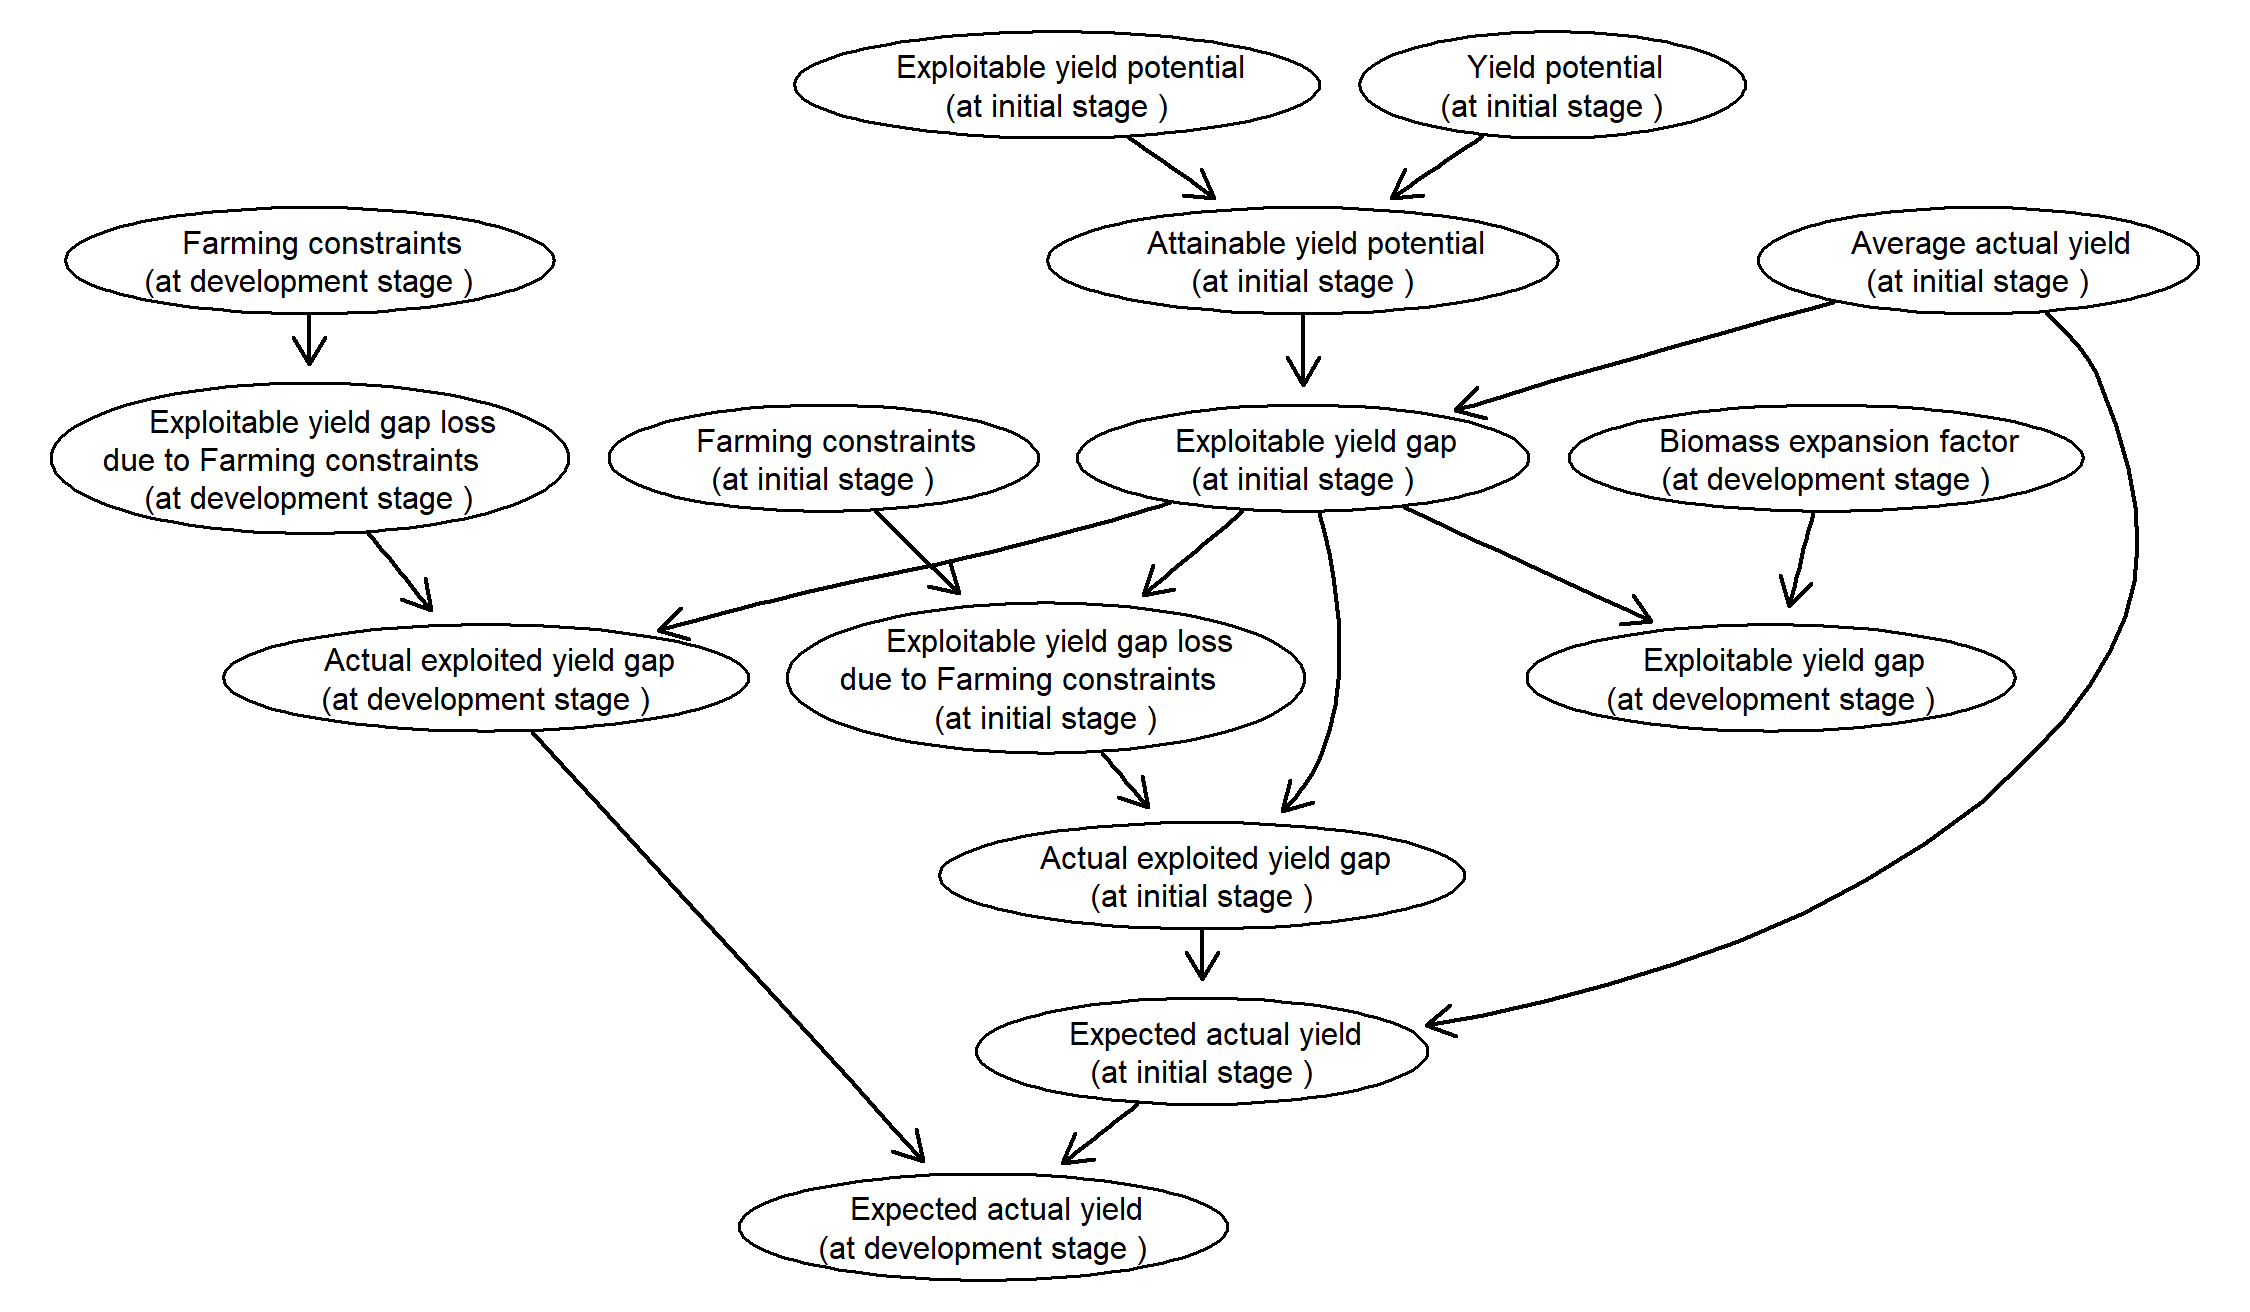
\includegraphics[width=1\linewidth,]{figures/figure_s9} 

}

\caption{Monte Carlo model describing important variables as part of a mixed model describing the expected crop yield at different stages of crop development in flood-based farming systems in Kisumu County (Kenya) and Tigray (Ethiopia).}\label{fig:fig9}
\end{figure}

We modelled biomass accumulation (i.e.~the amount of above-ground biomass produced by crops on a given farm) following the crop development, and ultimately converted biomass into grain yield using a realistic range of possible harvest index values. The maximum attainable biomass yield (Attainable yield potential) depends on the potential crop yield (Yield potential) and its achievable limit (Exploitable yield potential). This concept acknowledges that it is impossible for farmers to fully eliminate the farming constraints. The exploitable yield gap is then estimated by subtracting the long-term average yield (Average actual yield) from the attainable yield. Yield opportunity losses (Exploitable yield gap), therefore, are proportional to the difference in input allocation among farmers (Farming constraints) relative to the exploitable yield gap. Therefore, additional yield opportunity for a given farmer (Actual exploited yield gap) can be estimated by subtracting the yield opportunity loss from the exploitable yield gap. Finally, farm yield (Expected actual yield) can be obtained by adding the yield opportunity to the average yield.

\hypertarget{refs5}{%
\section{Rationales and objectives of the case studies}\label{refs5}}

\hypertarget{refs51}{%
\subsection{Assessment of soil water using the soil water module}\label{refs51}}

FBFS are possible solutions to the challenges of high rainfall variability and drought risk that characterize rainfed agriculture in many places, because they can harness additional water sources for supplementary irrigation. To resolve potential drought risk, farmers must store enough flood water in soils without creating lasting anaerobic conditions that would be detrimental for crops. This requires maximizing water storage in soils, while limiting waterlogging and restricting water losses through evaporation, run-off or percolation. In FBFS, drought and waterlogging depend heavily on the amount of floodwater reaching the plot, and water losses are inversely related to the quality and quantity of soil organic amendments and other intrinsic soil properties, as well as climatic factors. Depending on the soil type, farmers optimize soil water at plot level by diverting the desired amount of floodwater, sometimes in combination with manure application and tillage (e.g.~ploughing / rotavating). While most farmers use one or more soil and water conservation techniques, we encountered limited understanding of which techniques are most effective. The objective of this case study (sections \textbf{\emph{2.7. Inputs, outputs and special models}} and \textbf{\emph{3.2. Soil water module}} of the main paper) is to demonstrate how the generic model can be customized to prescribe optimum pre-season cultural practices for improved soil water on specific soil types using the soil water module in the BN sub-model.

\hypertarget{refs52}{%
\subsection{Probabilistic assessment of crop biomass using the crop growth module}\label{refs52}}

Apart from their substantial contribution to food security, FBFS also provide extensive amounts of fodder and post-harvest grazing opportunities for livestock in many areas. In both the Tigray region and Kisumu County, livestock feed on crop residues and other flood recession grasses, which make substantial contributions to livestock production. The symbiotic relationship between crops and livestock is well known and common to many farming systems. While crop biomass makes a substantial contribution to livestock production, most crop models focus their attention on grain yields, often failing to consider biomass yield at all. This case study (sections \textbf{\emph{2.7. Inputs, outputs and special models}} and \textbf{\emph{3.4. Crop growth module}} of the main paper) provides a purely probabilistic attempt towards using the crop growth module for assessing the expected biomass yield and other important biomass yield metrics (e.g.~biomass yield gap, exploited biomass yield). By providing these estimates at different stages of crop development, this instance of the generic model may also serve as a monitoring tool for biomass accumulation over the growing season.

\hypertarget{refs53}{%
\subsection{Impact of soil water and biotic stresses on grain yield of rice and sorghum}\label{refs53}}

Many important risk factors that affect farms (e.g.~pests, diseases and weeds) are ignored by many crop models, because they are either difficult to measure or too complex to include. The stochastic nature of many risk factors makes them difficult to predict with accuracy. In many agricultural settings, water, weeds, and pests and diseases rank among the top concerns and are perceived by farmers as major impediments to agricultural production. This is particularly important for FBFS, where the type of water management can strongly affect yield losses due to pests, diseases and weeds. Crop spacing can have a strong influence on the skills required of farmers for adequate management of biotic stressors. For example, weed removal in tef can be difficult and time-consuming compared to sorghum, which is traditionally planted in relatively sparse rows. Weed seeds can be washed onto fields by the flood water, along with moisture that creates suitable conditions for their germination and growth. In most FBFS, therefore, farmers must protect their crops at every stage against a host of biotic stressors. This becomes challenging when the available labour force is limited, in which case a farmer must prioritize certain crop protection activities over others. Such prioritization should be based on comparative analysis of plausible outcomes for different scenarios. The objective of this case study (sections \textbf{\emph{2.7. Inputs, outputs and special models}} and \textbf{\emph{3.5. Management module}} of the main paper) is to demonstrate how the model can be customized for use in assessments of the relative impacts of the top three yield-related concerns of farmers in the study area.

\hypertarget{references}{%
\section*{References}\label{references}}
\addcontentsline{toc}{section}{References}

\hypertarget{refs}{}
\leavevmode\hypertarget{ref-Cullen_and_Frey_1999}{}%
Cullen, A., Frey, C., 1999. Probabilistic Techniques in Exposure Assessment. Plenum Press, New York.

\leavevmode\hypertarget{ref-Delignette-Muller_and_Dutang_2015}{}%
Delignette-Muller, M.L., Dutang, C., 2015. fitdistrplus : An R Package for Fitting Distributions. Journal of Statistical Software 64, 1--34. \url{https://doi.org/10.18637/jss.v064.i04}

\leavevmode\hypertarget{ref-Luedeling_Goehring_et_al_2019}{}%
Luedeling, E., Goehring, L., Schiffers, K., 2019. decisionSupport: Quantitative support of decision making under uncertainty. The Comprehensive R Archive Network.

\hypertarget{acknowledgements}{%
\section*{Acknowledgements}\label{acknowledgements}}
\addcontentsline{toc}{section}{Acknowledgements}

This study was jointly funded by the \href{https://www.daad.de/en/}{Deutscher Akademischer Austauschdienst} (German Academic Exchange Service; DAAD) and the \href{http://www.worldagroforestry.org/}{World Agroforestry Centre} (International Centre for Research in Agroforestry; ICRAF). We thank the farmers and experts who contributed in various ways during the development of the model. We thank the department of Dryland Agriculture of Mekelle University for guidance on the sampling frame in the Tigray region and for facilitating logistics during field work. Thanks to the participants of the leadership course in flood-based farming and water harvesting in Kenya and the participants of the International Training on Integrated Watershed Management and FBFS in Ethiopia, who drafted the models.


\end{document}


